\subsection{Numerical Stability of the IFCG Algorithms}
\label{sec:ifcg_stability}
The main issue with the numerical stability of IFCG algorithms is the same as the one displayed by many other Krylov-based methods: The way the residual vector $r$ is computed.
It is usually done by just updating the residual of iteration $i$ from the one in iteration $i-1$ via expressions like $r_{i} = r_{i-1} - \alpha~Ap_{i-1}$.
However, by doing so, residual $r_{i}$ may deviate from the true residual $b-Ax_{i}$.
State-of-the-art approaches use a residual replacement strategy to prevent the updated residual $r_{i}$ to deviate from the true residual.
The remedy is to periodically replace the updated $r_{i}$ 
by $b-Ax_{i}$~\cite{carson, vorst99, ghysels14}.
The frequency of such replacement is a trade-off between convergence speed and accuracy and some sophisticated strategies exist 
~\cite{demmel14, vorst99} to deal with it. 
In the case of IFCG and IFCG2 
we do the $r_{i} = b-Ax_{i}$ replacement every \emph{FUSE} iterations to avoid hurting the overlap between different iterations.

We run some experiments considering several sparse matrices obtained from the Florida Sparse Matrix Collection~\cite{florida}.
These experiments involve parallel executions of the IFCG1, IFCG2, Pipelined CG and Preconditioned CG algorithms on a 16 cores NUMA node composed of two 8-core sockets.
More specific details on the parallel implementations and the precise 
experimental setup can be found in sections~\ref{sec:ifcg_implementation} and~\ref{sec:ifcg_setup}, respectively.
Also, Table~\ref{table:ifcg_matrices} contains a description of the matrices considered in the experiments.

\begin{figure}[bhtp]
	\centerline{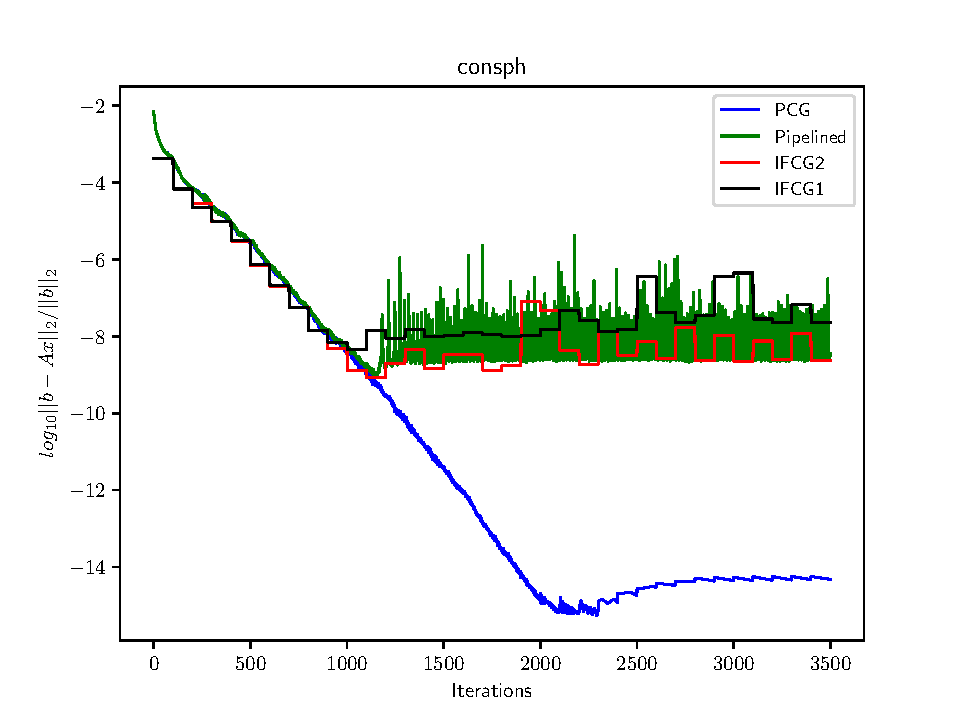
\includegraphics[scale=0.70]{ifcg/figs/mt_prec/cg_history_consph.pdf}}
	\vspace{-0.4cm}
	\caption{Convergence of the Preconditioned CG, Pipelined CG, IFCG1 and IFCG2 algorithms. Data regarding IFCG1 and IFCG2 is reported every 100 iterations since \emph{FUSE} = 100.}
	\label{prec}
	\vspace{-0.4cm}
\end{figure}


Figure \ref{prec} displays the evolution of the relative residual $||b-Ax_{i}||_{2}/||b||_{2}$ on matrix~\emph{consph} considering the IFCG1, IFCG2, Pipe\-lined CG and Preconditioned CG methods.
Data concerning IFCG1 and IFCG2 are expressed in a coarser-grain pattern than Pipelined and Preconditioned CG's data points since we calculate the relative residual every 100 iterations (i. e. \emph{FUSE}=100).
We can see that the convergence of the IFCG1 and IFCG2 algorithms is the same as Pipelined CG.
Interestingly, Figure~\ref{prec} also displays how the basic Preconditioned CG algorithm has better convergence properties than Pipelined CG, which is consistent with previously reported numerical results~\cite{ghysels14, cools16}.
We omit results concerning the rest of the matrices in Table~\ref{table:matrices} since they exhibit the exact same behavior as the one observed with ~\emph{consph}.
Our experiments show how the numerical behavior in terms of the relative residual $||b-Ax_{i}||_{2}/||b||_{2}$ achieved by IFCG1 and IFCG2 matches the state-of-the-art. 
\begin{figure*}[bhtp]
        \centerline{
                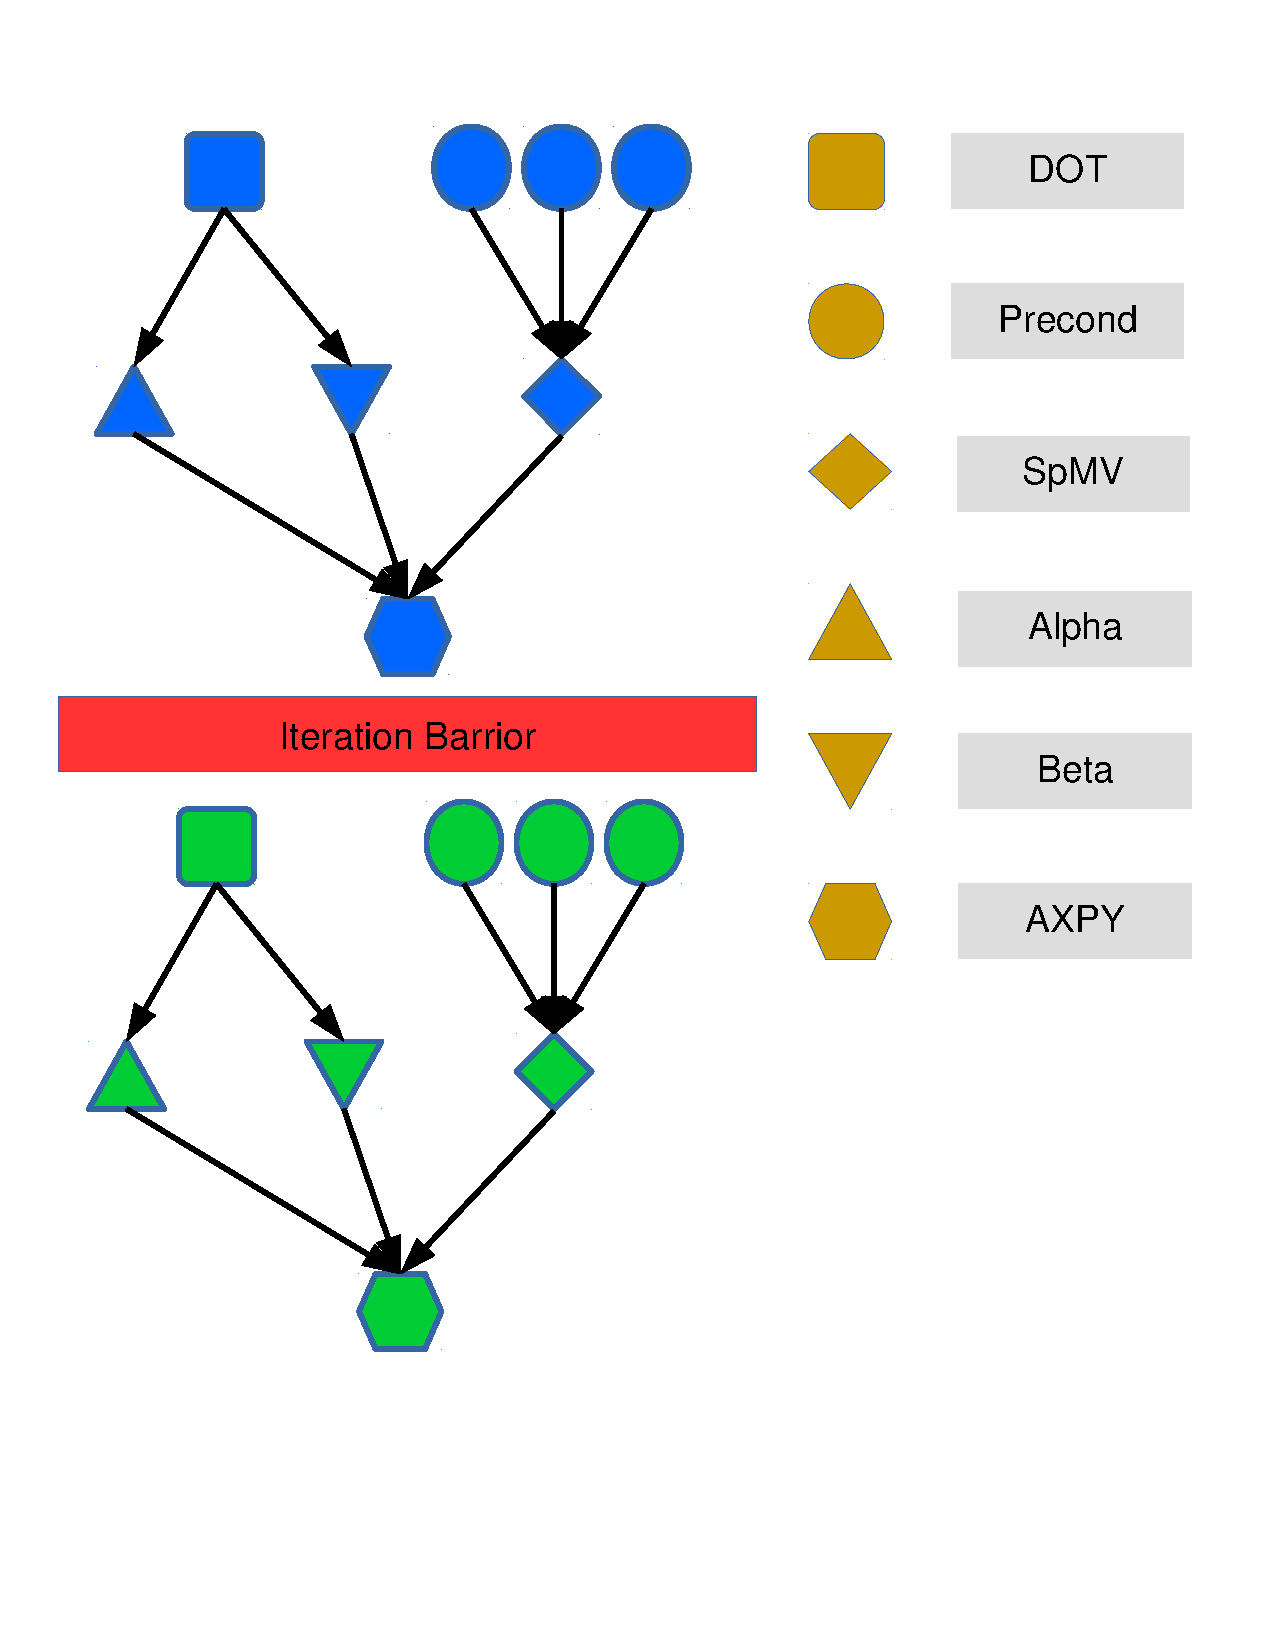
\includegraphics[scale=0.30]{ifcg/figs/charts/pcg.pdf}
                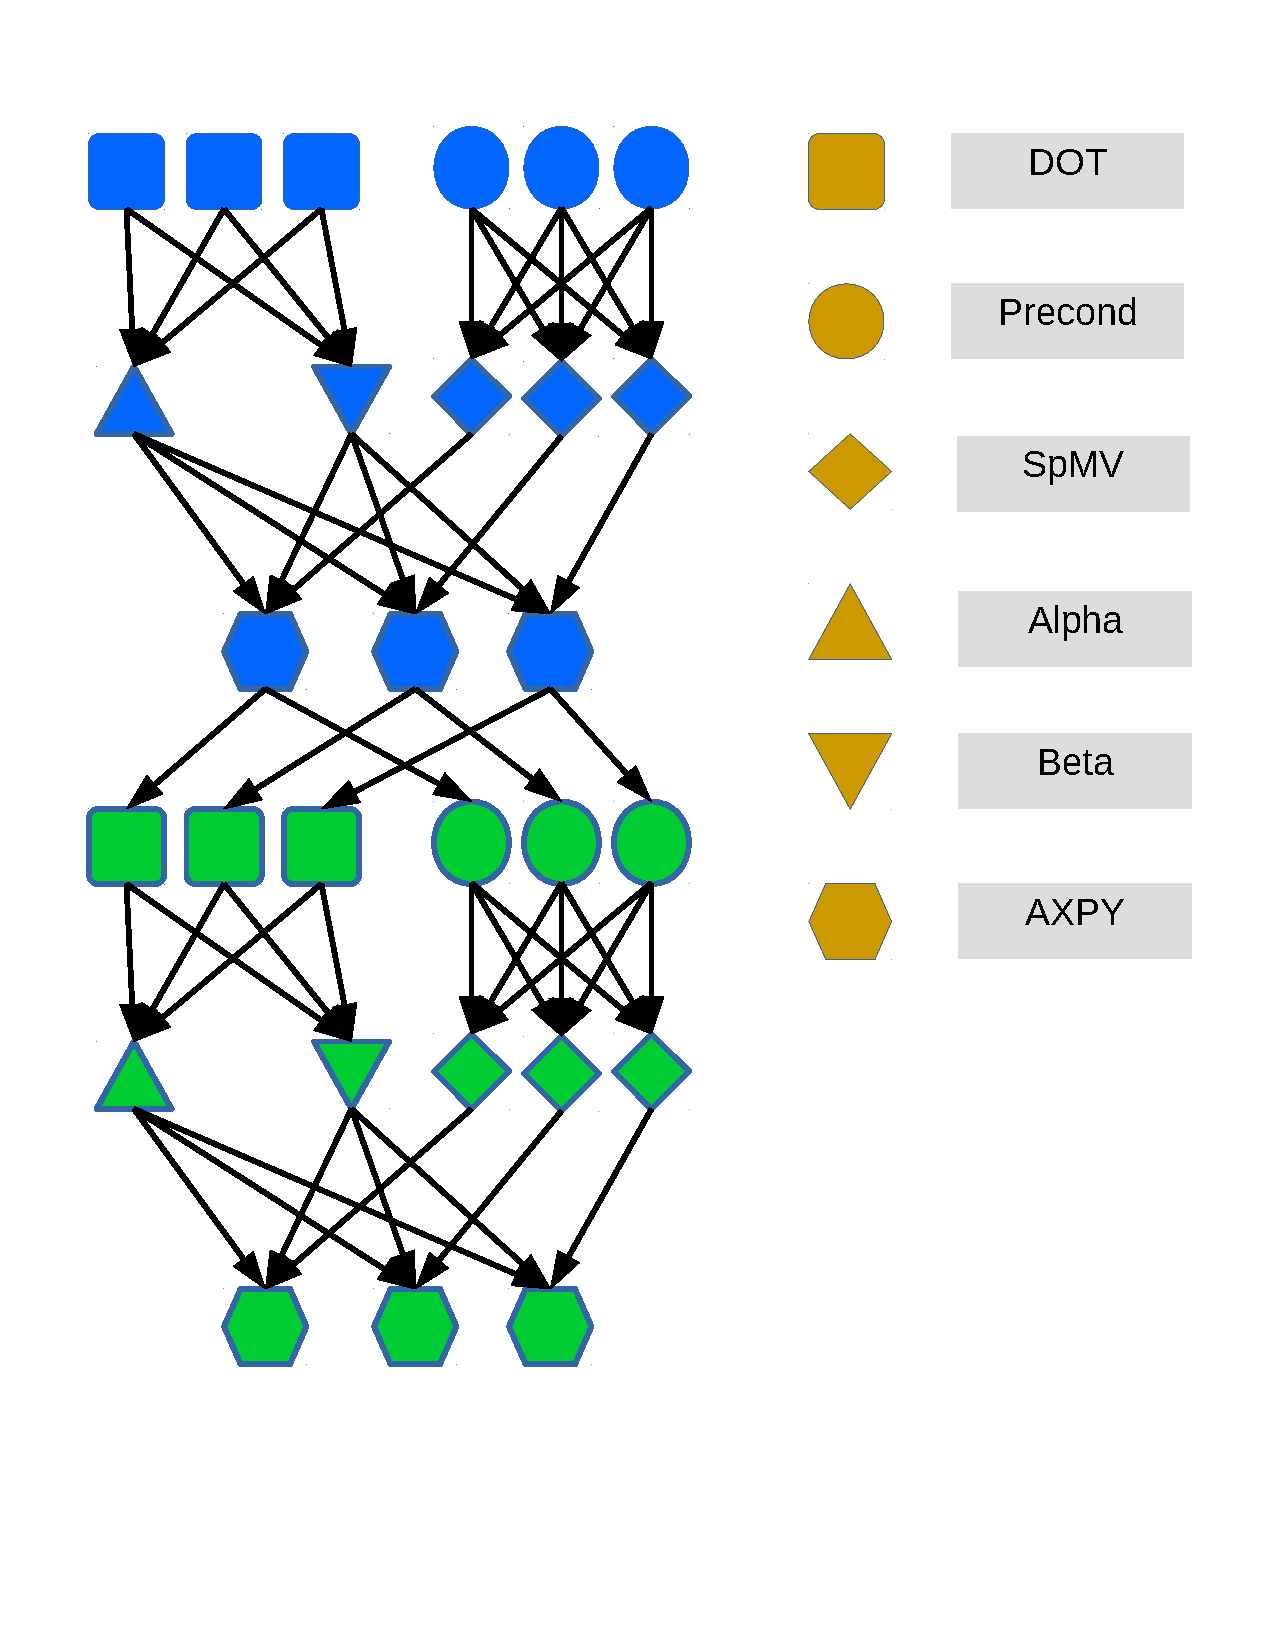
\includegraphics[scale=0.30]{ifcg/figs/charts/ifcg.pdf}
                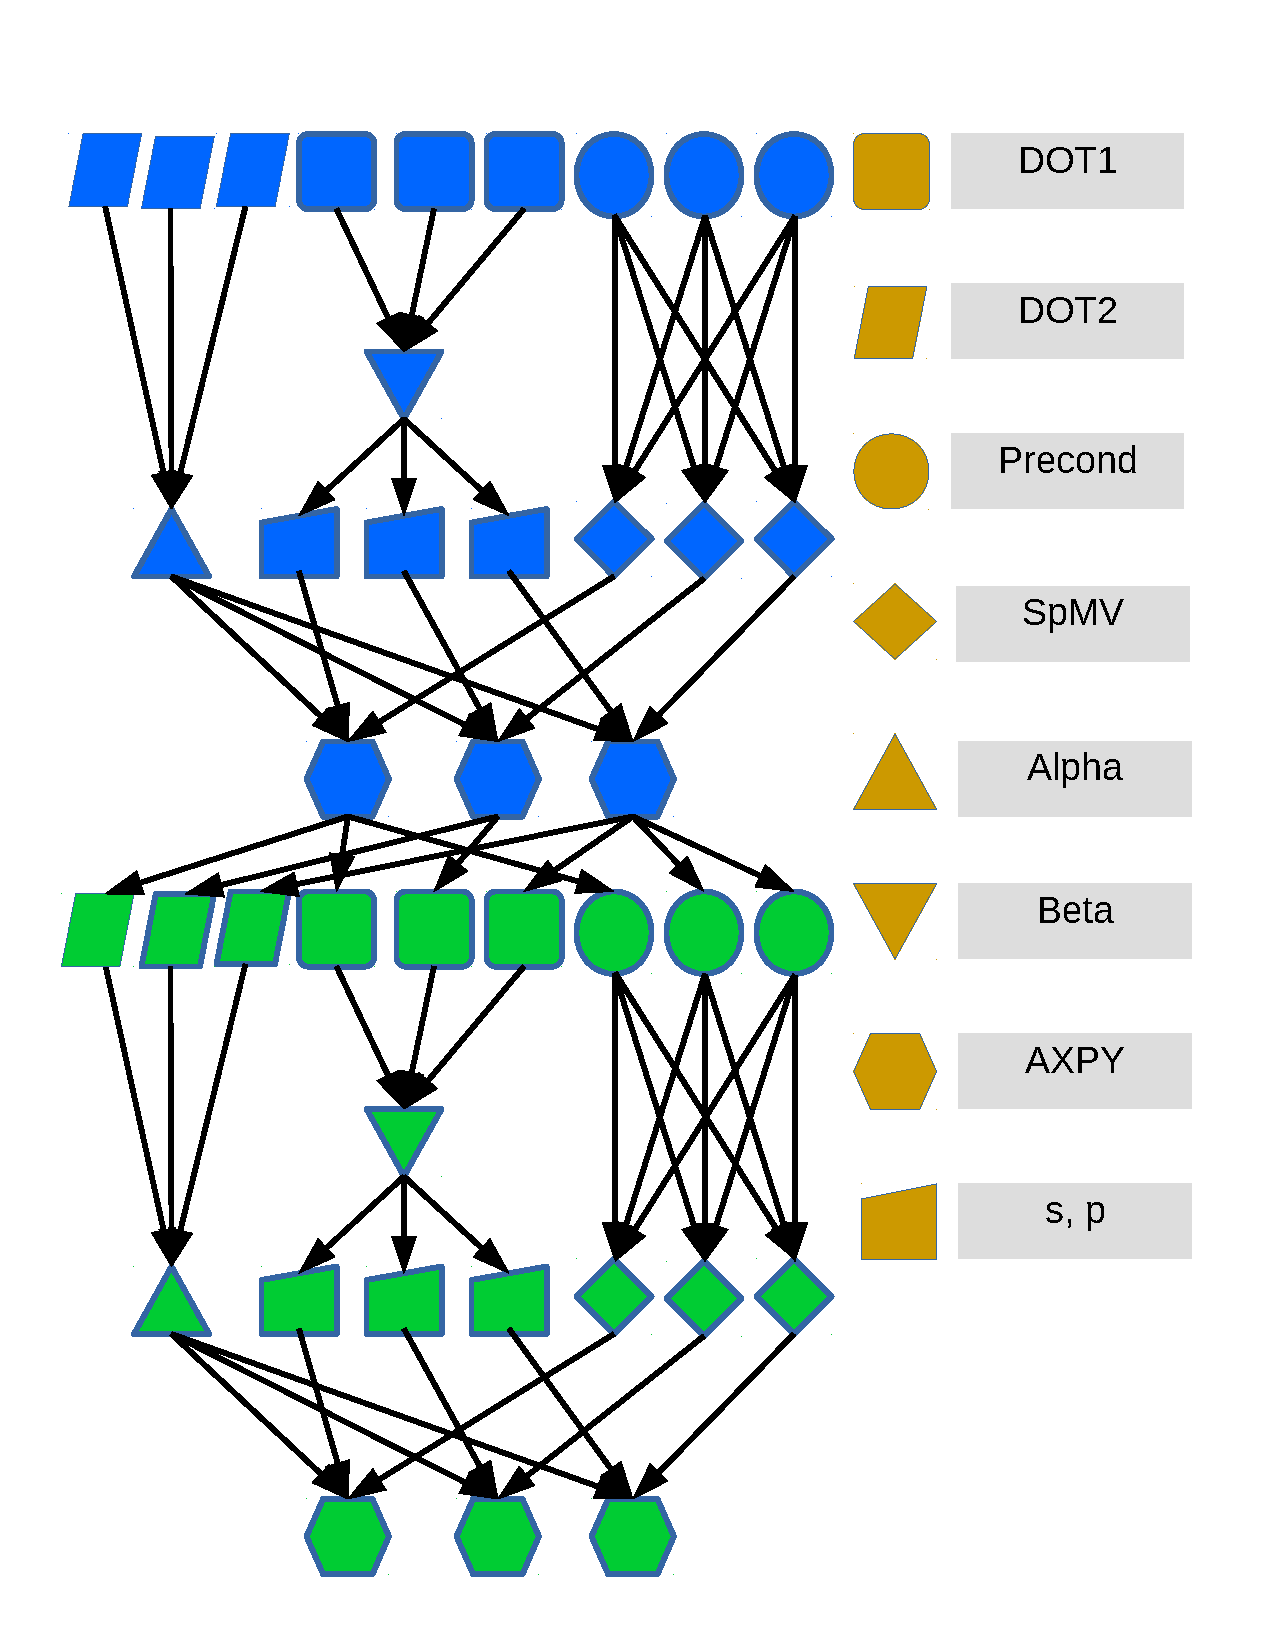
\includegraphics[scale=0.30]{ifcg/figs/charts/ifcg2.pdf}
        }
        \vspace{-0.6cm}
        \caption{Graphs of tasks representing two Iterations of Pipelined CG (left), IFCG1 (center) and IFCG2 (right), $N=3$.}
        \label{tdg}
\end{figure*}

\subsection{Parallel Execution of the IFCG Algorithms}
\label{sec:ifcg_implementation}

The IFCG algorithms have been carefully designed to hide the impact of their global synchronization points by overlapping them with other numerical kernels.
Also, IFCG algorithms aim at relaxing data-dependencies between these different kernels by breaking them down into several subkernels that just require a reduced input data set to carry on.
These features can significantly improve performance but, in order to exploit them,
the IFCG algorithms must run in parallel and enforce the overlap of the different computational kernels as much as possible.
Therefore, we need to specify at the source code level a parallel scheme that meets these requirements
and there are several ways to do so. 

One option is to statically specify at the application source code level the way different kernels overlap with each other, which should be done by means of sophisticated parallel programming techniques like pools of threads or active waiting loops that trigger work once its input data is ready.
%The usage of such techniques is indeed a possibility although their optimality is tightly related to the parallel hardware.
However, the optimality of these techniques depends a lot on the parallel hardware where the parallel execution takes place.
Therefore, a static approach is not practical since it needs to be adapted to each parallel execution scenario.
In this paper we follow a dynamic approach that conceives the parallel execution as a directed acyclic graph where the nodes represent pieces of code (also known as tasks) and the edges are control or data dependencies between them.
This approach requires from the programmer to specify the pieces of code or tasks that run in parallel by means of annotations that contain their input or output dependencies.
A runtime system orchestrates the parallel run by considering tasks' input or control dependencies and scheduling them into the available parallel hardware once all dependencies are satisfied.
The most important shared-memory programming models, like OpenMP, have support for this kind of task-based parallelism
and there is also support for running task-based workloads on distributed memory environments~\cite{Bueno13}. 

\subsection{Task-based Formulations of the Pipelined CG and IFCG algorithms} 
\label{sec:ifcg_task}

The Pipelined CG, IFCG1 and IFCG2 algorithms can be easily formulated in terms of tasks by just looking at each one of the steps in algorithms~\ref{alg:pcg},~\ref{alg:ifcg} and~\ref{alg:ifcg2} and considering them tasks. 
Indeed, by means of the \#pragma annotations provided by OpenMP it is possible to specify that each one of these steps is a task as well as which are its data dependencies.
Control dependencies are typically expressed in terms of sentinels.
Importantly, IFCG1 and IFCG2 have many more tasks per iteration than Pipelined CG.
Indeed, steps 3-6 and 12-19 of Pipeline CG ({\bf Algorithm~\ref{alg:pcg}}) 
are split into $N$ substeps in {\bf Algorithms~\ref{alg:ifcg} and~\ref{alg:ifcg2}}, which implies that we have $N$ tasks in IFCG1 and IFCG2 per each Pipeline CG task.  
The only exception to this rule is the preconditioning step which is typically split depending on whether or not the chosen preconditioner allows a decomposition in terms of tasks.

Figure~\ref{tdg} shows two iterations of the Pipelined CG, IFCG1 and IFCG2 algorithms represented in terms of task graphs.
Parameter $N$ is equal to $3$, which means that many of the Pipelined CG tasks appearing in the task graph are broken down
into 3 tasks by the IFCG1 and IFCG2 methods.
In the case of the Pipelined CG algorithm the task named \emph{DOT} represents steps 3 and 4 of {\bf Algorithm~\ref{alg:pcg}} while tasks named \emph{Precond} represents step 5, which in this particular case is divided into several tasks. 
Tasks $\alpha$ and $\beta$ represent the computations done within step 8.
Finally, the task designated as \emph{AXPY} represents steps 12-19.
Similarly, the task graph representations of the IFCG1 and IFCG2 methods represent all the steps displayed by algorithms~\ref{alg:ifcg}-\ref{alg:ifcg2}.

By comparing the center and the left hand side task graphs in Figure~\ref{tdg} we can observe how by removing the iteration barrier and breaking the computation routines into 
blocks we expose much more parallelism to the hardware. 
Indeed, Pipelined CG has a limited potential for overlapping tasks belonging to the same iteration and cannot overlap tasks from different iterations at all since its inter-iteration barrier prevents it from doing so.
In contrast, IFCG1 displays a much more flexible parallel pattern that can easily overlap tasks belonging to different iterations.
IFCG2, by further extracting two AXPYs operations (s, p) that only depend on $\beta$, is able to create even more concurrency.
The implications and analysis of these varying level of parallelism shown by the different algorithms are explained in Section~\ref{sec:ifcg_results}.

\begin{table}[H]
\fontsize{9}{9}\selectfont
\centering
\resizebox{.80\textwidth}{!}{  
\begin{tabular}{|c|c|c|c|}
\hline
\textbf{Name} & \textbf{Dimension} & \textbf{Nonzeros} & \textbf{Nonzeros\%}\\
\hline \hline
G3\_circuit & 1585478 & 7660826 & 0.0003\% \\
\hline
thermal2 & 1228045 & 8580313 & 0.0006\% \\
\hline
ecology2 & 999999 & 4995991 & 0.0005\% \\
\hline
af\_shell8 & 504855 & 17579155 & 0.0068\% \\
\hline
G2\_circuit & 150102 & 726674 & 0.003\% \\
\hline
cfd2 & 123440 & 3085406 & 0.02\% \\
\hline
consph & 83334 & 6010480 & 0.087\% \\
\hline
%nd24k & 72000 & 28715634 & 55.4\% \\
%\hline
\end{tabular}
}
\vspace{0.2cm}
\caption{Matrices used for experiments}
\label{table:ifcg_matrices}
\vspace{-0.5cm}
\end{table}
